\subsection{Amplificatore differenziale}

\begin{wrapfigure}[14]{l}{0.5\textwidth}
  \begin{center}
    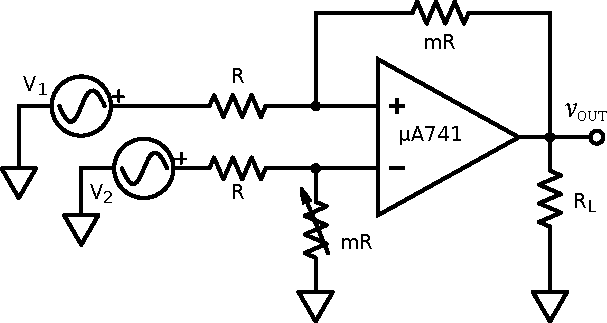
\includegraphics[width=0.33\textwidth]{../E05/latex/c_teo_diff_amp.pdf}
  \end{center}
  \caption{Grafico teorico di un amplificatore differenziale. Per $m$ si intende un fattore moltiplicativo rispetto alla $R$.}
  \label{cir5:diff_amp_teo}
\end{wrapfigure}

In questa parte dell'esperienza cercheremo di capire e analizzare un amplificatore differenziale, il cui schema circuitale è in Figura \ref{cir5:diff_amp}. Oltre al fatto che scegliendo i valori di resistenza possiamo decidere il guadagno, la proprietà più importante è sicuramente l'abbattimento del rumore di modo comune. Per capirne il motivo analizziamo il circuito teorico riportato in Figura \ref{cir5:diff_amp_teo}.

Sfruttiamo il principio di sovrapposizione per valutare la tensione in uscita in funzione delle due di ingresso, ricordandoci che tale principio può essere applicato per sistemi lineari: ciò è molto utile in quanto ci permette di separare l'analisi circuitale e ricondurci a casi più semplici.

Chiamiamo $V^-$ la tensione all'ingresso invertente e $V^+$ quella all'ingresso non invertente. Analizziamo prima il caso in cui $V_1=0$. La tensione nel punto $V_+$ sarà data dal partitore con $R$ ed $mR$ (verso l'op-amp non scorre corrente). Assumendo l'op-amp ideale, abbiamo $V^+=V^-$. Possiamo dunque scrivere:

\begin{equation}
\begin{cases} V_+=V_-  \\ V_+=V_2\frac{mR}{R+mR} \\ V_-= V_{out2}\frac{R}{R+mR}\end{cases}  \Rightarrow V_{out2}=mV_2
\label{eq 5: vout2}
\end{equation}

Analogamente, poniamo $V_2=0$. Otteniamo le seguenti equazioni del circuito:

\begin{equation}
\begin{cases} V_+=V_-=0  \\ \frac{V_1}{R}+\frac{V_{out2}}{mR}=0 \end{cases}  \Rightarrow V_{out1}=-mV_1
\label{eq 5: vout1}
\end{equation}

Sommando ora (\ref{eq 5: vout2}) e (\ref{eq 5: vout2}) otteniamo $V_{out}=m(V_2-V_1)$.

Possiamo ora passare ad analizzare il circuito da cui siamo partiti, ovvero quello affetto da noise (da noi simulato con un'onda sinusoidale) riportato in Figura \ref{cir5:diff_amp}. Valgono dunque le seguenti equazioni

%\begin{center}
$$
\begin{cases} V_1=V_{in}+V_{noise} \\ V_2=V_{noise} \end{cases}  \Rightarrow V_{out}=m(V_{noise}-(V_{in}+V_{noise}))=-V_{in}
$$
%\end{center}

L'amplificatore differenziale ci permette dunque di eliminare in modo efficace il rumore di modo comune. 

Inoltre, abbiamo posto come resistenza collegata tra comune e $V_+$ un trimmer per impostare la tensione di modo comune al più basso valore possibile. Infatti, le resistenze non sono in realtà esattamente uguali e prima di utilizzare il circuito è necessario bilanciarlo in modo da ottenere un segnale il più piccolo possibile quando i segnali in ingresso sono uguali.

\begin{wrapfigure}[17]{r}{0.5\textwidth}
  \begin{center}
    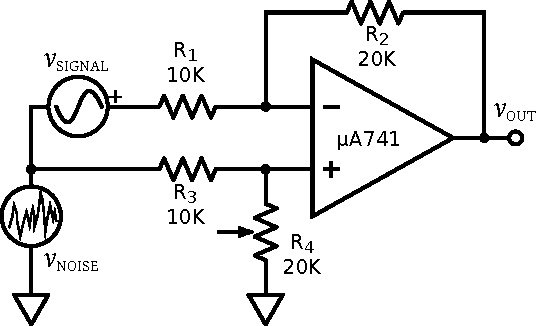
\includegraphics[width=0.33\textwidth]{../E05/latex/c_diff_amp.pdf}
  \end{center}
  \caption{Grafico dell'amplificatore differenziale utilizzato durante l'esperienza. $R_4$ è un trimmer multigiro di resistenza variabile.}
  \label{cir5:diff_amp}
\end{wrapfigure}

In laboratorio abbiamo utilizzato come sorgente di noise il generatore di forme d'onda e come $V_{in}$ il generatore di tensione costante. Abbiamo utilizzato delle R da \SI{10}{\kilo\ohm} e $mR=2R$. La resistenza variabile è stata costruita mettendo in serie una da \SI{10}{\kilo\ohm} con un trimmer, anch'esso da \SI{10}{\kilo\ohm}. Per controllare il bilanciamento abbiamo connesso entrambi gli ingressi al generatore di forme d'onda ed è stato utilizzato un segnale sinusoidale di $20Vpp$. Il segnale in uscita è stato dunque riportato sull'oscilloscopio. Abbiamo notato che, cambiando il valore della resistenza con il trimmer, il segnale in uscita variava. Il miglior bilanciamento che siamo riusciti a raggiungere ha portato la tensione picco-picco del rumore a \SI{0.5}{\milli\volt}. Abbiamo dunque posto come segnale in entrata un valore costante di tensione con il generatore di tensione costante, e alimentato il circuito con $-2Vpp$. Il rumore è sempre stato simulato con una sinusoidale di $20Vpp$. Questo risultato è riportato in Figura \ref{gr5:amp_diff}.

Come vediamo, il rumore è stato completamente eliminato dall'amplificatore differenziale. Abbiamo successivamente provato a sbilanciare il circuito, per vedere l'effetto del rumore sul segnale in uscita. E' stata dunque variata la resistenza con trimmer e abbiamo utilizzato un rumore con dei picchi molto accentuati, così da vedere bene gli effetti sul segnale in uscita (l'output è in Figura \ref{gr5:sbil_amp_diff}). 

\begin{figure}[ht]
 \centering
   {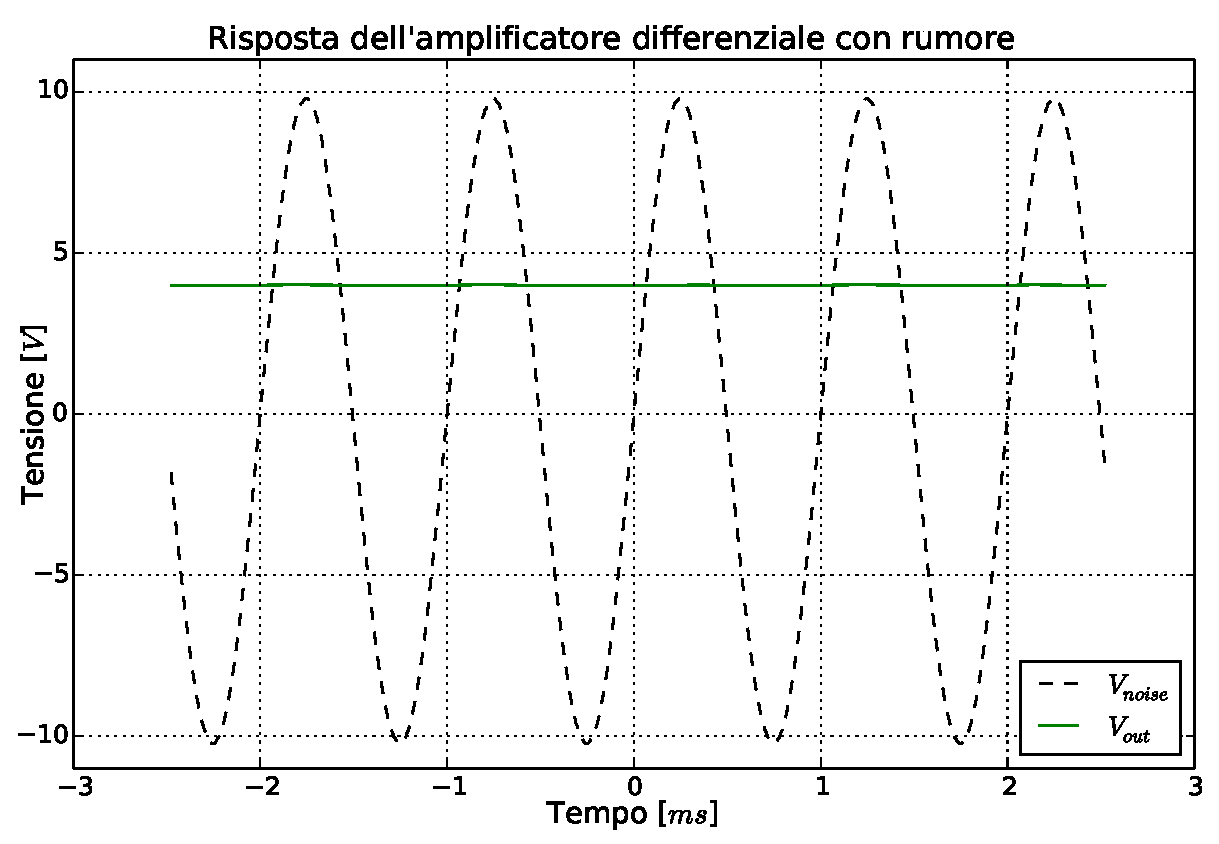
\includegraphics[width=0.85\textwidth]{../E05/latex/amp_diff.pdf}}
 \caption{Come vediamo dal grafico, il rumore che abbiamo simulato ha un'ampiezza di 20 Volt picco-picco (sinusoide in nero). Nonostante ciò, l'uscita (in verde) non è affatto influenzata e risulta amplificata di 2 volte, come stimato precedentemente dai calcoli teorici. }
 \label{gr5:amp_diff}
\end{figure}

\begin{figure}[ht]
 \centering
   {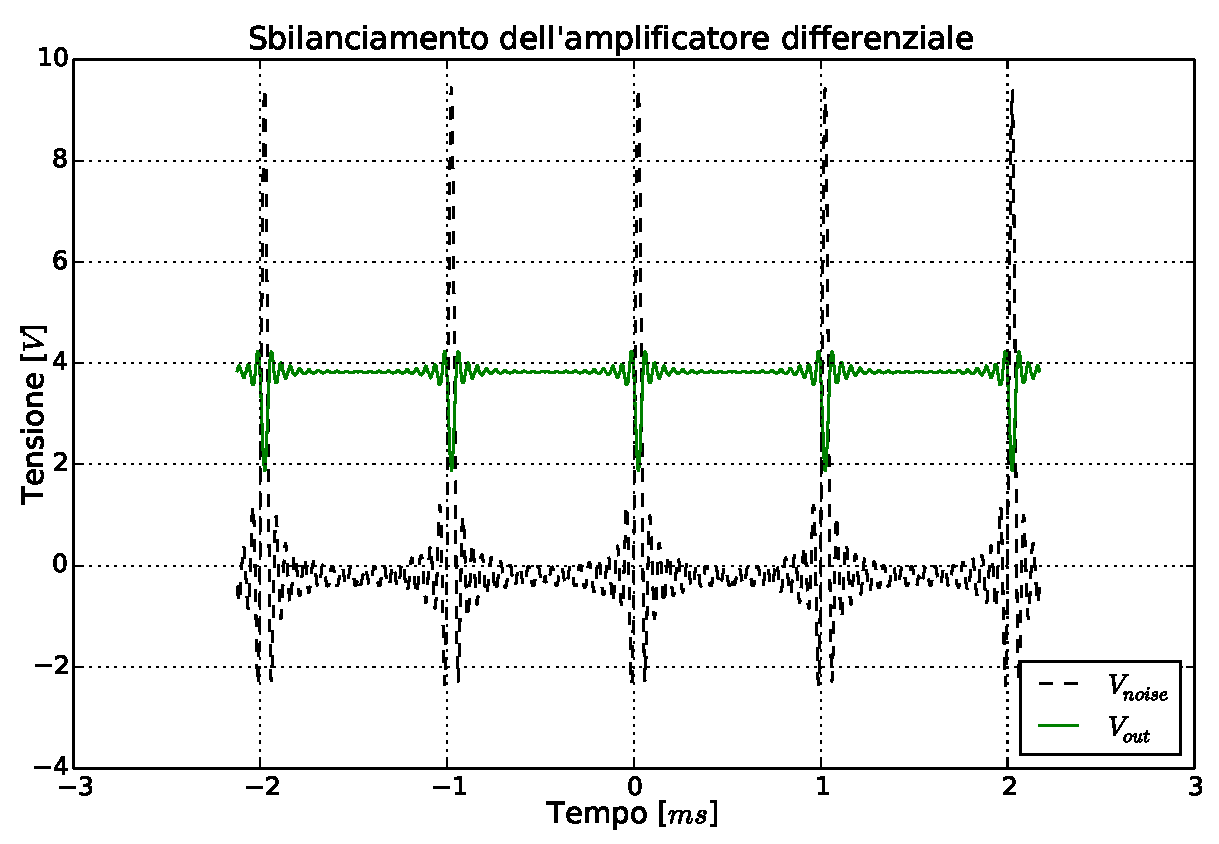
\includegraphics[width=0.85\textwidth]{../E05/latex/sbil_amp_diff.pdf}}
 \caption{Dopo lo sbilanciamento del circuito non è più garantita la soppressione del rumore in modo comune. Come vediamo, il segnale in uscita risulta distorto. E' dunque necessario calibrare bene il circuito prima di effettuare esperimenti nei quali si vuole eliminare un rumore comune ad entrambi i segnali in ingresso.}
 \label{gr5:sbil_amp_diff}
\end{figure}

Inoltre, il guadagno può essere cambiato solo se si cambiano 2 resistenze nel circuito. Una soluzione efficace che inoltre rimedia alla bassa impedenza in ingresso è quella di utilizzare un Amplificatore per Strumentazione, il cui funzionamento è esposto al paragrafo successivo.